% Template for PLoS
% Version 3.5 March 2018
%
% % % % % % % % % % % % % % % % % % % % % %
%
% -- IMPORTANT NOTE
%
% This template contains comments intended 
% to minimize problems and delays during our production 
% process. Please follow the template instructions
% whenever possible.
%
% % % % % % % % % % % % % % % % % % % % % % % 
%
% Once your paper is accepted for publication, 
% PLEASE REMOVE ALL TRACKED CHANGES in this file 
% and leave only the final text of your manuscript. 
% PLOS recommends the use of latexdiff to track changes during review, as this will help to maintain a clean tex file.
% Visit https://www.ctan.org/pkg/latexdiff?lang=en for info or contact us at latex@plos.org.
%
%
% There are no restrictions on package use within the LaTeX files except that 
% no packages listed in the template may be deleted.
%
% Please do not include colors or graphics in the text.
%
% The manuscript LaTeX source should be contained within a single file (do not use \input, \externaldocument, or similar commands).
%
% % % % % % % % % % % % % % % % % % % % % % %
%
% -- FIGURES AND TABLES
%
% Please include tables/figure captions directly after the paragraph where they are first cited in the text.
%
% DO NOT INCLUDE GRAPHICS IN YOUR MANUSCRIPT
% - Figures should be uploaded separately from your manuscript file. 
% - Figures generated using LaTeX should be extracted and removed from the PDF before submission. 
% - Figures containing multiple panels/subfigures must be combined into one image file before submission.
% For figure citations, please use "Fig" instead of "Figure".
% See http://journals.plos.org/plosone/s/figures for PLOS figure guidelines.
%
% Tables should be cell-based and may not contain:
% - spacing/line breaks within cells to alter layout or alignment
% - do not nest tabular environments (no tabular environments within tabular environments)
% - no graphics or colored text (cell background color/shading OK)
% See http://journals.plos.org/plosone/s/tables for table guidelines.
%
% For tables that exceed the width of the text column, use the adjustwidth environment as illustrated in the example table in text below.
%
% % % % % % % % % % % % % % % % % % % % % % % %
%
% -- EQUATIONS, MATH SYMBOLS, SUBSCRIPTS, AND SUPERSCRIPTS
%
% IMPORTANT
% Below are a few tips to help format your equations and other special characters according to our specifications. For more tips to help reduce the possibility of formatting errors during conversion, please see our LaTeX guidelines at http://journals.plos.org/plosone/s/latex
%
% For inline equations, please be sure to include all portions of an equation in the math environment.  For example, x$^2$ is incorrect; this should be formatted as $x^2$ (or $\mathrm{x}^2$ if the romanized font is desired).
%
% Do not include text that is not math in the math environment. For example, CO2 should be written as CO\textsubscript{2} instead of CO$_2$.
%
% Please add line breaks to long display equations when possible in order to fit size of the column. 
%
% For inline equations, please do not include punctuation (commas, etc) within the math environment unless this is part of the equation.
%
% When adding superscript or subscripts outside of brackets/braces, please group using {}.  For example, change "[U(D,E,\gamma)]^2" to "{[U(D,E,\gamma)]}^2". 
%
% Do not use \cal for caligraphic font.  Instead, use \mathcal{}
%
% % % % % % % % % % % % % % % % % % % % % % % % 
%
% Please contact latex@plos.org with any questions.
%
% % % % % % % % % % % % % % % % % % % % % % % %

\documentclass[10pt,letterpaper]{article}
\usepackage[top=0.85in,left=2.75in,footskip=0.75in]{geometry}

% amsmath and amssymb packages, useful for mathematical formulas and symbols
\usepackage{amsmath,amssymb}

% Use adjustwidth environment to exceed column width (see example table in text)
\usepackage{changepage}

% For commenting
\usepackage{comment}

% Use Unicode characters when possible
\usepackage[utf8x]{inputenc}

% textcomp package and marvosym package for additional characters
\usepackage{textcomp,marvosym}

% cite package, to clean up citations in the main text. Do not remove.
\usepackage{cite}

% Use nameref to cite supporting information files (see Supporting Information section for more info)
\usepackage{nameref,hyperref}

% line numbers
\usepackage[right]{lineno}

% ligatures disabled
\usepackage{microtype}
\DisableLigatures[f]{encoding = *, family = * }

% color can be used to apply background shading to table cells only
\usepackage[table]{xcolor}

% array package and thick rules for tables
\usepackage{array}

% create "+" rule type for thick vertical lines
\newcolumntype{+}{!{\vrule width 2pt}}

% create \thickcline for thick horizontal lines of variable length
\newlength\savedwidth
\newcommand\thickcline[1]{%
  \noalign{\global\savedwidth\arrayrulewidth\global\arrayrulewidth 2pt}%
  \cline{#1}%
  \noalign{\vskip\arrayrulewidth}%
  \noalign{\global\arrayrulewidth\savedwidth}%
}

% \thickhline command for thick horizontal lines that span the table
\newcommand\thickhline{\noalign{\global\savedwidth\arrayrulewidth\global\arrayrulewidth 2pt}%
\hline
\noalign{\global\arrayrulewidth\savedwidth}}


% Remove comment for double spacing
%\usepackage{setspace} 
%\doublespacing

% Text layout
\raggedright
\setlength{\parindent}{0.5cm}
\textwidth 5.25in 
\textheight 8.75in

% Bold the 'Figure #' in the caption and separate it from the title/caption with a period
% Captions will be left justified
\usepackage[aboveskip=1pt,labelfont=bf,labelsep=period,justification=raggedright,singlelinecheck=off]{caption}
\renewcommand{\figurename}{Fig}

% Use the PLoS provided BiBTeX style
\bibliographystyle{plos2015}

% Remove brackets from numbering in List of References
\makeatletter
\renewcommand{\@biblabel}[1]{\quad#1.}
\makeatother



% Header and Footer with logo
\usepackage{lastpage,fancyhdr,graphicx}
\usepackage{epstopdf}
%\pagestyle{myheadings}
\pagestyle{fancy}
\fancyhf{}
%\setlength{\headheight}{27.023pt}
%\lhead{\includegraphics[width=2.0in]{PLOS-submission.eps}}
\rfoot{\thepage/\pageref{LastPage}}
\renewcommand{\headrulewidth}{0pt}
\renewcommand{\footrule}{\hrule height 2pt \vspace{2mm}}
\fancyheadoffset[L]{2.25in}
\fancyfootoffset[L]{2.25in}
\lfoot{\today}

%% Include all macros below

\newcommand{\lorem}{{\bf LOREM}}
\newcommand{\ipsum}{{\bf IPSUM}}

%% END MACROS SECTION


\begin{document}
\vspace*{0.2in}

% Title must be 250 characters or less.
\begin{flushleft}
{\Large
\textbf\newline{Membrane-localized Keratin-14 Promotes Invasion} % Please use "sentence case" for title and headings (capitalize only the first word in a title (or heading), the first word in a subtitle (or subheading), and any proper nouns).
}
\newline
% Insert author names, affiliations and corresponding author email (do not include titles, positions, or degrees).
\\
Yohannes Tsehay\textsuperscript{1},
Hildur Knutsodottir\textsuperscript{1},
Andrei Kucharavy\textsuperscript{1\textcurrency},
Veena Padmanaban\textsuperscript{2},
Joel Bader\textsuperscript{1*}
%with the Lorem Ipsum Consortium\textsuperscript{\textpilcrow}
\\
\bigskip
\textbf{1} High-Throughout Biology Center and Department of Biomedical Engineering, Johns Hopkins University, Baltimore, MD, USA
\\
\textbf{2} Center for Cell Dynamics and Department of Cell Biology, Johns Hopkins University School of Medicine, Baltimore, MD, USA
\\
\bigskip

% Insert additional author notes using the symbols described below. Insert symbol callouts after author names as necessary.
% 
% Remove or comment out the author notes below if they aren't used.
%
% Primary Equal Contribution Note
%\Yinyang These authors contributed equally to this work.

% Additional Equal Contribution Note
% Also use this double-dagger symbol for special authorship notes, such as senior authorship.
%\ddag These authors also contributed equally to this work.

% Current address notes
\textcurrency Current Address: Dept/Program/Center, Institution Name, City, State, Country % change symbol to "\textcurrency a" if more than one current address note
% \textcurrency b Insert second current address 
% \textcurrency c Insert third current address

% Deceased author note
%\dag Deceased

% Group/Consortium Author Note
%\textpilcrow Membership list can be found in the Acknowledgments section.

% Use the asterisk to denote corresponding authorship and provide email address in note below.
* joel.bader@jhu.edu

\end{flushleft}
% Please keep the abstract below 300 words
\section*{Abstract}
Metastasis is the main predictor of outcome for patients with cancer, yet the molecular mechanism driving invasive phenotypes is not well under-stood, hindering development of assays and therapeutics for this stage of cancer progression. In this study, we characterize a molecular biomarker for invasion in greater detail, using an automated computer model. The model quantifies the invasive potential of tumors, allowing for quantification of even minor contributions to an invasive phenotype from individual genes, and can potentially be used to establish interactions among genes. Keratin 14 (K14) is a known molecular biomarker that is correlated with poor outcomes in breast cancer patients. We apply our automated computer model, which was built in Python, to test the hypothesis that K14 is directly correlated with automatically generated invasion scores, independent of tumor size. We used two different transgenic mice as our breast cancer tumor models. Organoids were generated from these mice, and each organoid had a corresponding differential interference contrast image, K14 image, and a boundary around the organoid drawn manually which was used to generate an invasion score for the organoid using our automated system. The parameters assessed include the following: entire K14 expression, peripheral K14 expression (edges of the organoid), central K14 expression (center of the organoid), and organoid size. Peripheral K14 expression showed the strongest correlation with invasion scores for both types of transgenic mice, suggesting that K14 expression in cells located in the periphery may be an important marker of invasion. This relationship was more prominent in one mouse model than the other, indicating that additional factors play a role in invasion and dissemination. In future studies, we plan to perform a similar analysis using human organoids generated from breast tumors.


% Please keep the Author Summary between 150 and 200 words
% Use first person. PLOS ONE authors please skip this step. 
% Author Summary not valid for PLOS ONE submissions.   
\section*{Author summary}

\linenumbers

% Use "Eq" instead of "Equation" for equation citations.
\section*{Introduction}
%Lorem ipsum dolor sit~\cite{bib1} amet, consectetur adipiscing elit. Curabitur eget porta erat. Morbi consectetur est vel gravida pretium. Suspendisse ut dui eu ante cursus gravida non sed sem. Nullam Eq~(\ref{eq:schemeP}) sapien tellus, commodo id velit id, eleifend volutpat quam. Phasellus mauris velit, dapibus finibus elementum vel, pulvinar non tellus. Nunc pellentesque pretium diam, quis maximus dolor faucibus id.~\cite{bib2} Nunc convallis sodales ante, ut ullamcorper est egestas vitae. Nam sit amet enim ultrices, ultrices elit pulvinar, volutpat risus.

Alternative title: Morphological features of organoid invasion are correlated with membrane-localized Keratin-14 expression

\textcolor{blue}{
\begin{itemize}
    \item Biology intro (what is our audience). The two different mice models.
    \item How K14 expression is related to metastasis.
    \item The use of image analysis for feature extraction, lit review.
    \item Why spectral score is a good measure for invasion potential.
    \item Paper outline
\end{itemize}
}

Metastasis stats.

What are organoids.

Quantitative phenotypes.

Previous observation from Ewald group about K14 expression.

Hypothesis: a) K14 expression is correlated with organoid invasion.\\
b) organoid size is correlated with invasion score.

Research questions:

%\begin{eqnarray}
%\label{eq:schemeP}
%	\mathrm{P_Y} = \underbrace{H(Y_n) - H(Y_n|\mathbf{V}^{Y}_{n})}_{S_Y} + \underbrace{H(Y_n|\mathbf{V}^{Y}_{n})- %H(Y_n|\mathbf{V}^{X,Y}_{n})}_{T_{X\rightarrow Y}},
%\end{eqnarray}

\section*{Materials and methods}
\subsection*{Data acquisition}

 A total of 4 PyMT and 4 C31T mice were used to generate a total of \{\} organoids, which were then cultured in collagen I gels for 5 days. At day 5, they were imaged, an average of 16 per sample. Differential interference contrast (DIC) microscopy yielded 1040$\times$1388 pixel images. Microscope optics defined a resolution of 0.51190476 $\mu$m per pixel, corresponding to a 532.4$\times$710.5 $\mu$m field of view. Images were manually tracked in {\sc ImageJ} \cite{Schneider:2012ui} to define the organoid boundaries as pairs of points $\{x_v,y_v\}$ for $v \in [0,V-1]$. The total number of points $V$ depended on the manual tracking, and the spacing between adjacent points was similarly variable.

% For figure citations, please use "Fig" instead of "Figure".
% Nulla mi mi, Fig~\ref{fig1} venenatis sed ipsum varius, volutpat euismod diam. Proin rutrum vel massa non gravida. Quisque tempor sem et dignissim rutrum. Lorem ipsum dolor sit amet, consectetur adipiscing elit. Morbi at justo vitae nulla elementum commodo eu id massa. In vitae diam ac augue semper tincidunt eu ut eros. Fusce fringilla erat porttitor lectus cursus, \nameref{S1_Video} vel sagittis arcu lobortis. Aliquam in enim semper, aliquam massa id, cursus neque. Praesent faucibus semper libero.



% Results and Discussion can be combined.
\section*{Results}
% Nulla mi mi, venenatis sed ipsum varius, Table~\ref{table1} volutpat 

\begin{figure}[!h]
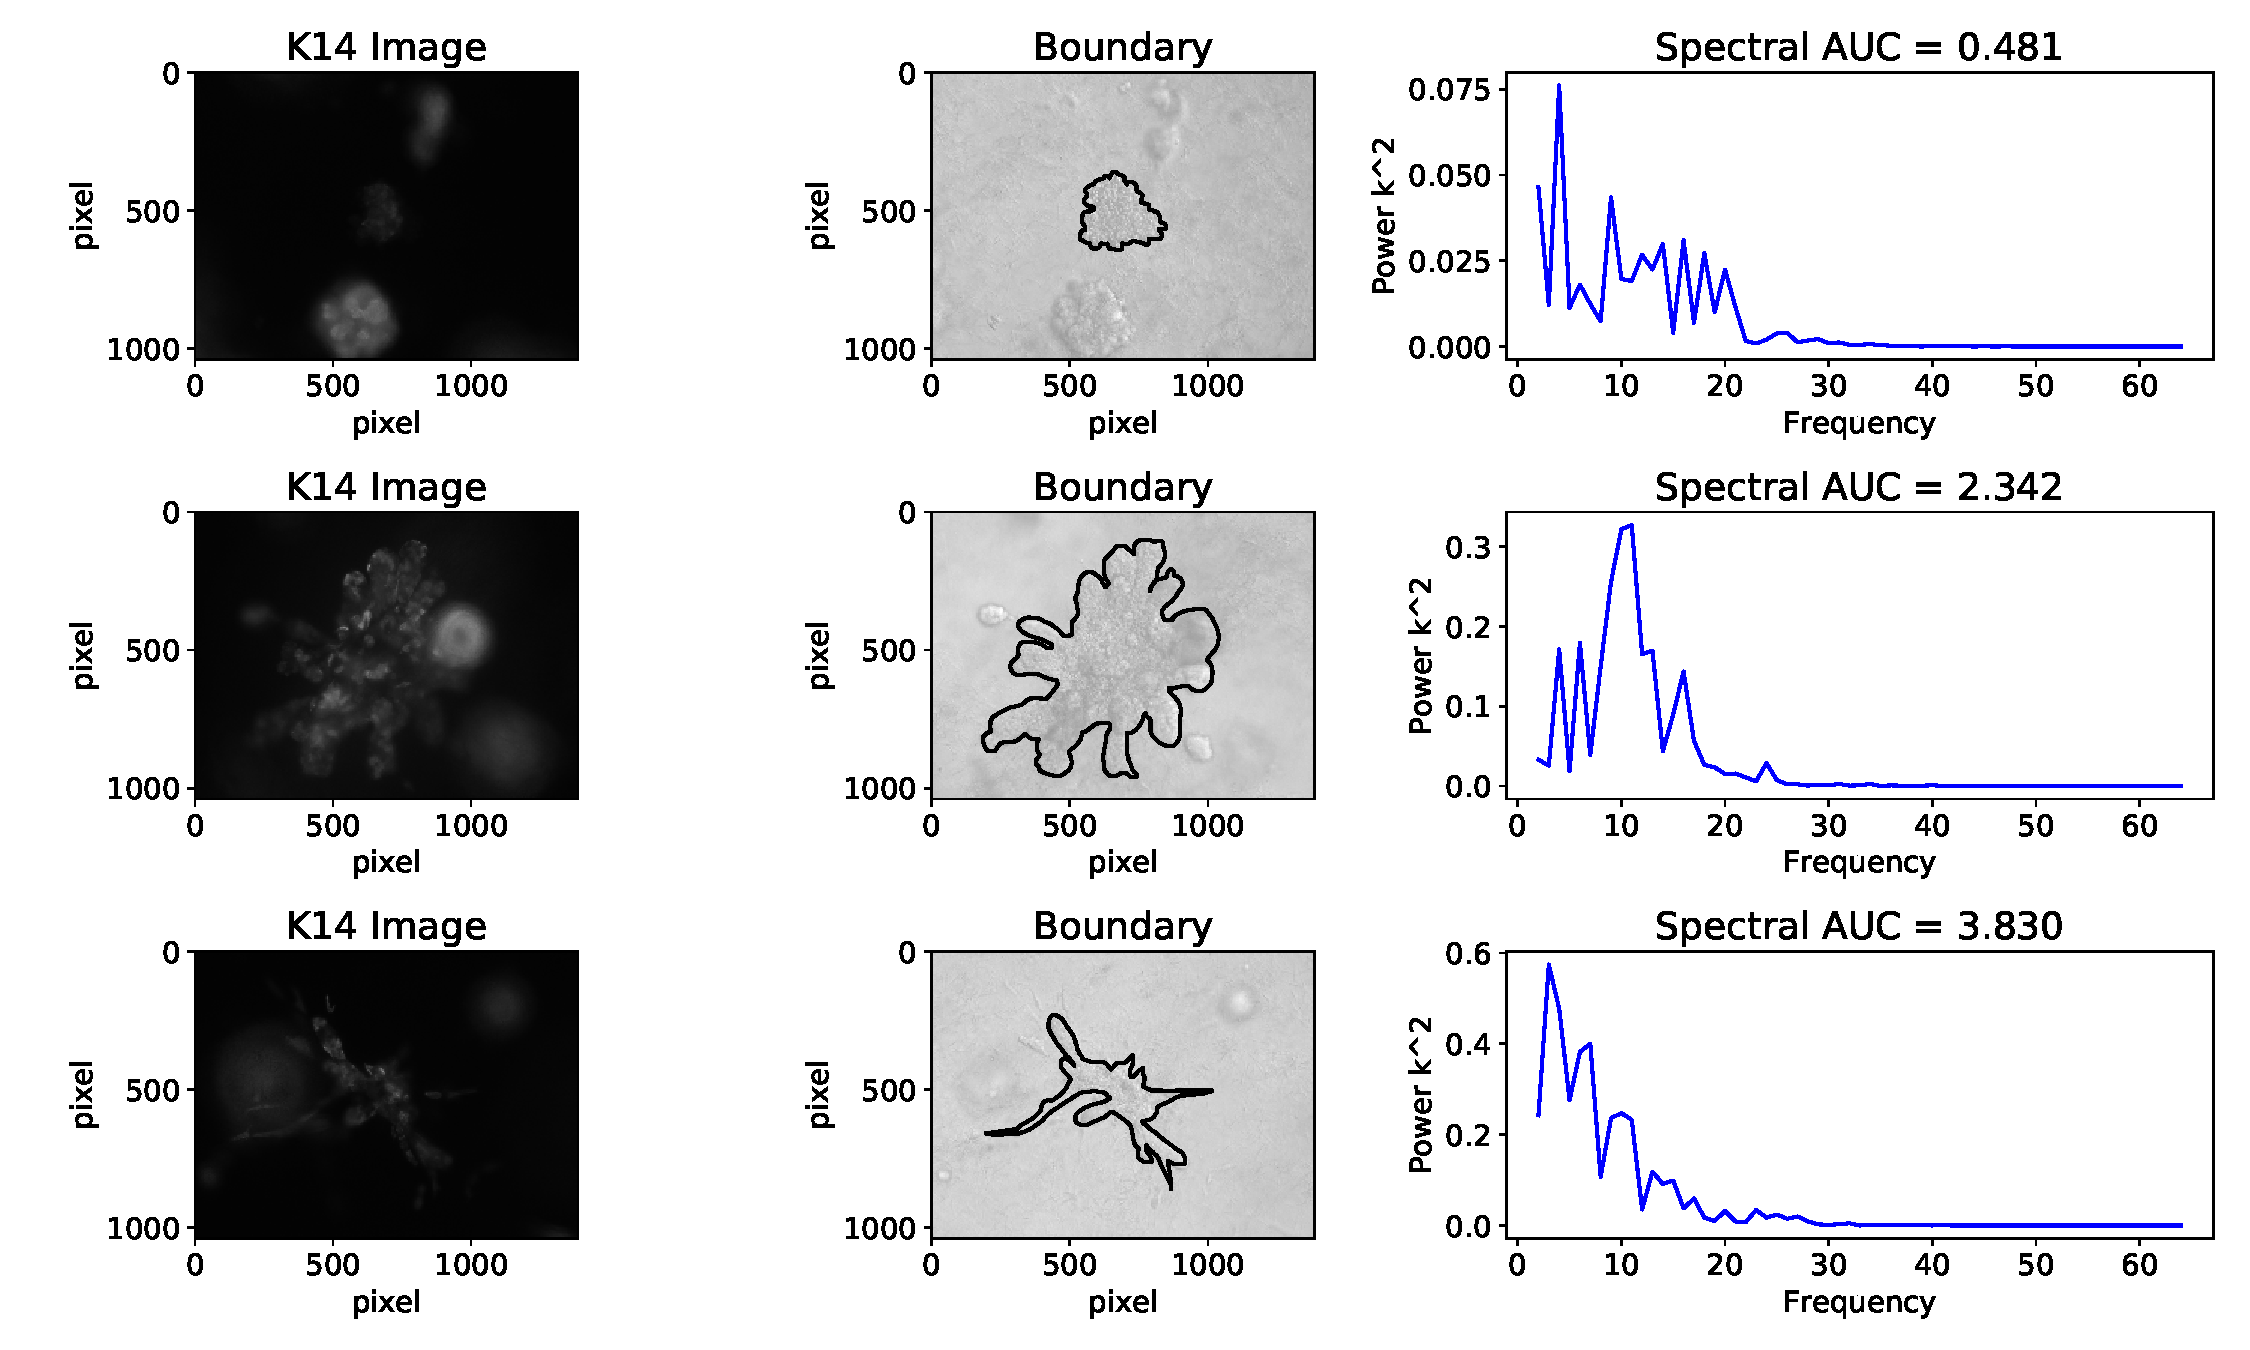
\includegraphics[width=\textwidth]{Image1.pdf}
\caption{Displays the K14 Image, DIC image, Bounday and spectral power analysis plots for three different organoids. \textcolor{red}{Axis font needs to be bigger. Y-axis in spectral score should all be the same and we can probably skip column 2.}} 
\label{fig1}
\end{figure}


\begin{figure}[!h]
\centering
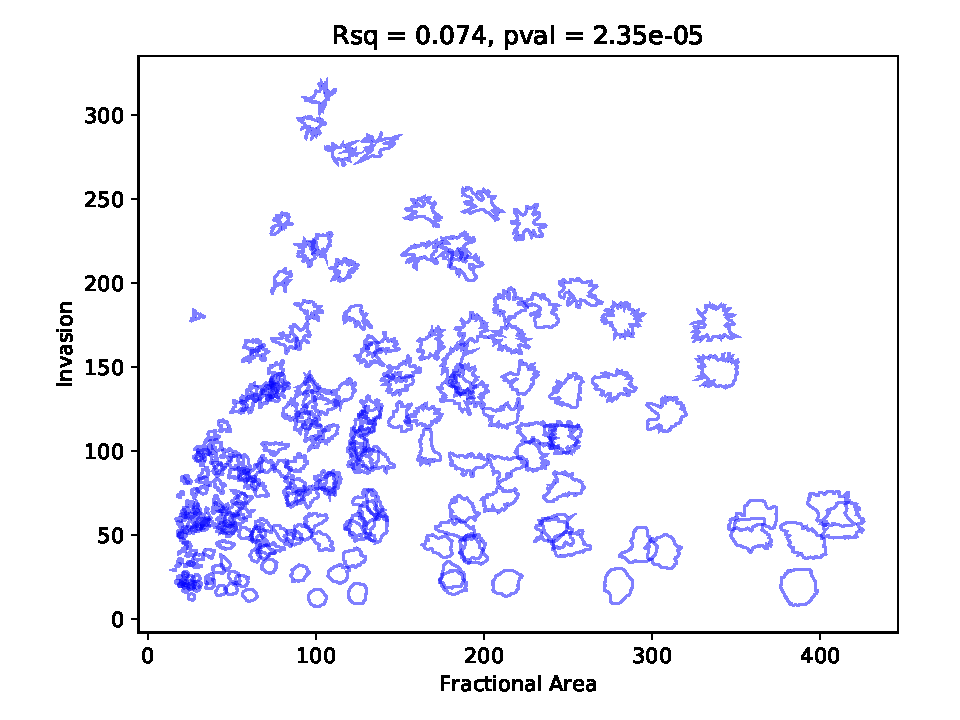
\includegraphics[width=\textwidth]{docs/01_paper/mouse_1_Day5_FA.pdf}
\caption{comment} 
\label{fig2}
\end{figure}

\begin{figure}[!h]
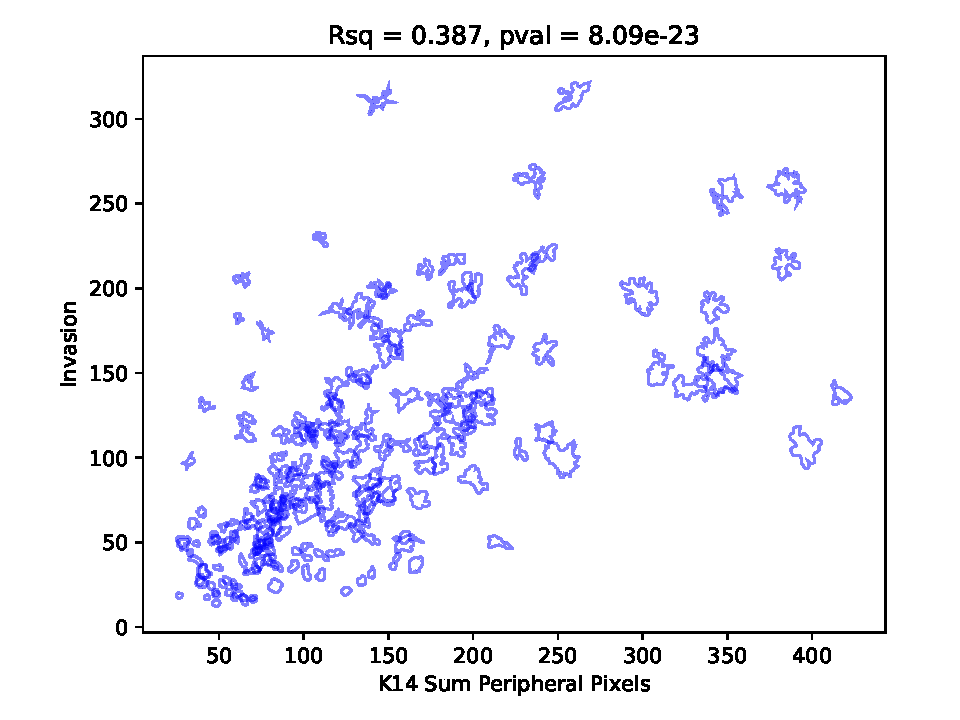
\includegraphics[width=\textwidth]{docs/01_paper/mouse_1_Day5_KPS.pdf}
\caption{comment} 
\label{fig3}
\end{figure}

\begin{figure}[!h]
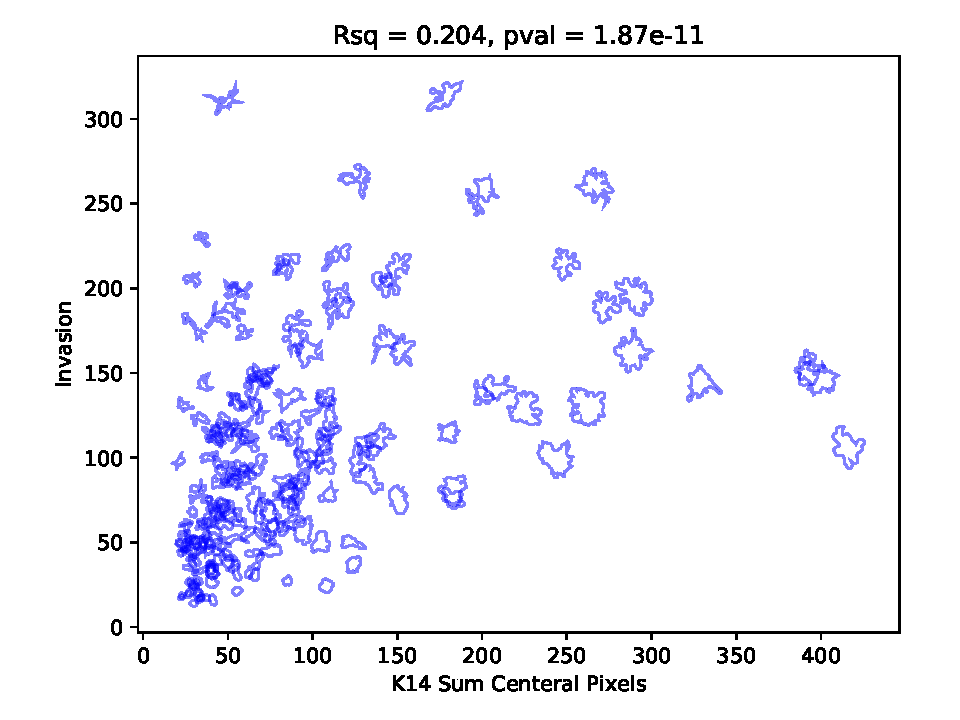
\includegraphics[width=\textwidth]{docs/01_paper/mouse_1_Day5_KCS.pdf}
\caption{comment} 
\label{fig4}
\end{figure}

\begin{figure}[!h]
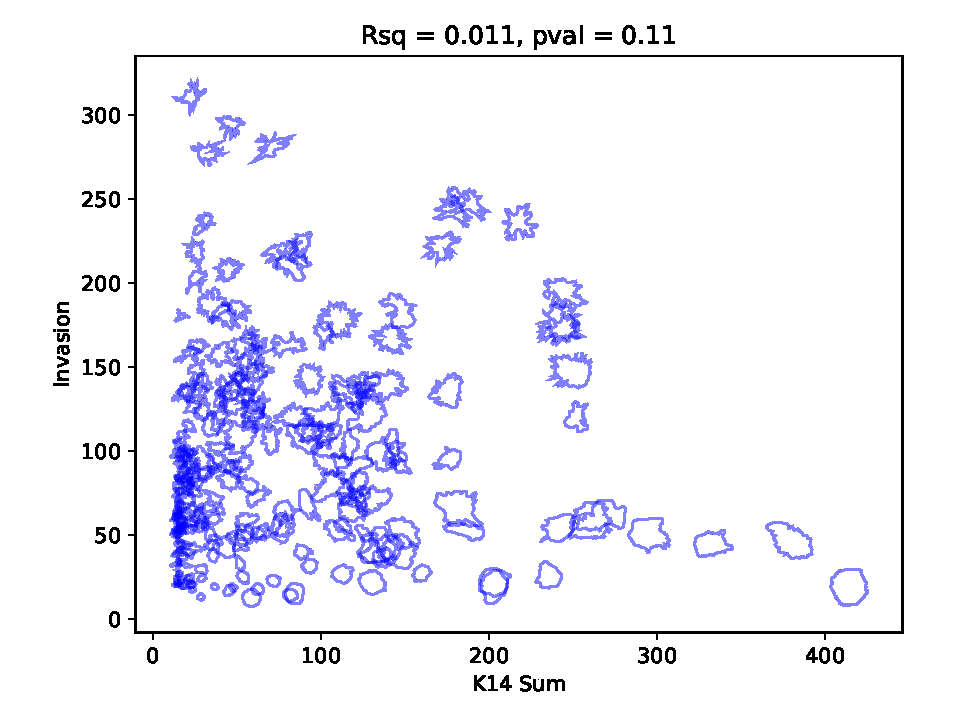
\includegraphics[width=\textwidth]{docs/01_paper/mouse_1_Day5_KS.pdf}
\caption{comment} 
\label{fig4}
\end{figure}

\begin{table}
\caption{{\bf Peripheral K14 explains correlates with invasive potential the best.}}
\label{tab1}
		\centering
		\resizebox{0.8\textwidth}{!}{
		 \begin{tabular}{||l c c c c||}
			\hline
			 & \multicolumn{4}{|c|}{$r^2$ by mouse} \\
			 \hline
			 Organoids (PyMMT mice) & 	1 & 2 & 3 & 4 \\ [0.5ex]
			 \hline\hline
			  \textbf{Peripheral sum K14} & \textbf{0.39} & \textbf{0.43} & \textbf{0.29} & \textbf{0.123} \\
			 \hline
			 Centeral sum K14 & 0.21 & 0.19 & 0.11 & 0.010 \\
			 \hline
			 Entire sum K14 & 0.22 & 0.22 & 0.12 & 0.013 \\
			 \hline
%			 K14 Mean & 0.02 & 0.04 & 0.03 \\ [1ex]
%			 \hline
			Organoid size & 0.27 & 0.33 & 0.27 & 0.076 \\
			 \hline
		\end{tabular}
		}
\end{table}

\begin{table}
\caption{{\bf Peripheral K14 explains correlates with invasive potential the best.}}
\label{tab1}
		\centering
		\resizebox{0.8\textwidth}{!}{
		 \begin{tabular}{||l c c c c||}
			\hline
			 & \multicolumn{4}{|c|}{$r^2$ by mouse} \\
			 \hline
			 Organoids (C3(1)tag mice) & 1 & 2 & 3 & 4  \\ [0.5ex]
			 \hline\hline
			  \textbf{Peripheral sum K14} & \textbf{0.11} & \textbf{0.25} & 0.06 & 0.03 \\
			 \hline
			 Centeral sum K14 & 0.01 & 0.03 & 0.06 & 0.00\\
			 \hline
			 Entire sum K14 & 0.01 & 0.00 & 0.01 & 0.00\\
			 \hline
%			 K14 Mean & 0.02 & 0.04 & 0.03 & xx\\ [1ex]
%			 \hline
			Organoid size & 0.07 & 0.01 & \textbf{0.07} &  \textbf{0.06} \\
			 \hline
		\end{tabular}
		}
\end{table}

Start adding figures here.\\
Q: Are we keeping the large vs. small organoids?
Q: should this be split into PyMT section and C31Tag section?

Fig. 1: show each step in the pipeline from DCI to spectral score for 2 organoids (one with low spectral score and one with high spectral score).

Fig. 2: show figures for the convolution kernel used to get peripheral K14 expression.

Fig. 3: Correlation plots PyMT

Fig. 4: Correlation plots C31Tag

Table 1: Summary statistics

\begin{comment}
% Place tables after the first paragraph in which they are cited.
\begin{table}[!ht]
\begin{adjustwidth}{-2.25in}{0in} % Comment out/remove adjustwidth environment if table fits in text column.
\centering
\caption{
{\bf Table caption Nulla mi mi, venenatis sed ipsum varius, volutpat euismod diam.}}
\begin{tabular}{|l+l|l|l|l|l|l|l|}
\hline
\multicolumn{4}{|l|}{\bf Heading1} & \multicolumn{4}{|l|}{\bf Heading2}\\ \thickhline
$cell1 row1$ & cell2 row 1 & cell3 row 1 & cell4 row 1 & cell5 row 1 & cell6 row 1 & cell7 row 1 & cell8 row 1\\ \hline
$cell1 row2$ & cell2 row 2 & cell3 row 2 & cell4 row 2 & cell5 row 2 & cell6 row 2 & cell7 row 2 & cell8 row 2\\ \hline
$cell1 row3$ & cell2 row 3 & cell3 row 3 & cell4 row 3 & cell5 row 3 & cell6 row 3 & cell7 row 3 & cell8 row 3\\ \hline
\end{tabular}
\begin{flushleft} Table notes Phasellus venenatis, tortor nec vestibulum mattis, massa tortor interdum felis, nec pellentesque metus tortor nec nisl. Ut ornare mauris tellus, vel dapibus arcu suscipit sed.
\end{flushleft}
\label{table1}
\end{adjustwidth}
\end{table}
\end{comment}


%PLOS does not support heading levels beyond the 3rd (no 4th level headings).
\subsection*{\lorem\ and \ipsum\ nunc blandit a tortor}
\subsubsection*{3rd level heading} 
 

\begin{enumerate}
	\item{react}
	\item{diffuse free particles}
	\item{increment time by dt and go to 1}
\end{enumerate}


\section*{Discussion}
%Nulla mi mi, venenatis sed ipsum varius, Table~\ref{table1} volutpat euismod diam. Proin rutrum vel massa non gravida. Quisque tempor sem et dignissim rutrum. Lorem ipsum dolor sit amet, consectetur adipiscing elit. Morbi at justo vitae nulla elementum commodo eu id massa. In vitae diam ac augue semper tincidunt eu ut eros. Fusce fringilla erat porttitor lectus cursus, vel sagittis arcu lobortis. Aliquam in enim semper, aliquam massa id, cursus neque. Praesent faucibus semper libero~\cite{bib3}.

We implemented a method to quanitfy the invasive phenotypes organoids derived from two distinct mouse models, namely PyMT and C3(1)tag.\\
Out of the features we tested, we found that peripheral K14 expression correlated with the invasive phenotype.\\
Why is this important and/or interesting?\\
Future directions: Test our method on Patient derived organoids, PDOs.\\
Does organoid invasion score correlate with patient outcome?

\section*{Conclusion}


\section*{Supporting information}

% Include only the SI item label in the paragraph heading. Use the \nameref{label} command to cite SI items in the text.
\paragraph*{S1 Fig.}
\label{S1_Fig}
{\bf Bold the title sentence.} Add descriptive text after the title of the item (optional).

\paragraph*{S2 Fig.}
\label{S2_Fig}
{\bf Lorem ipsum.} Maecenas convallis mauris sit amet sem ultrices gravida. Etiam eget sapien nibh. Sed ac ipsum eget enim egestas ullamcorper nec euismod ligula. Curabitur fringilla pulvinar lectus consectetur pellentesque.

\paragraph*{S1 File.}
\label{S1_File}
{\bf Lorem ipsum.}  Maecenas convallis mauris sit amet sem ultrices gravida. Etiam eget sapien nibh. Sed ac ipsum eget enim egestas ullamcorper nec euismod ligula. Curabitur fringilla pulvinar lectus consectetur pellentesque.

\paragraph*{S1 Video.}
\label{S1_Video}
{\bf Lorem ipsum.}  Maecenas convallis mauris sit amet sem ultrices gravida. Etiam eget sapien nibh. Sed ac ipsum eget enim egestas ullamcorper nec euismod ligula. Curabitur fringilla pulvinar lectus consectetur pellentesque.

\paragraph*{S1 Appendix.}
\label{S1_Appendix}
{\bf Lorem ipsum.} Maecenas convallis mauris sit amet sem ultrices gravida. Etiam eget sapien nibh. Sed ac ipsum eget enim egestas ullamcorper nec euismod ligula. Curabitur fringilla pulvinar lectus consectetur pellentesque.

\paragraph*{S1 Table.}
\label{S1_Table}
{\bf Lorem ipsum.} Maecenas convallis mauris sit amet sem ultrices gravida. Etiam eget sapien nibh. Sed ac ipsum eget enim egestas ullamcorper nec euismod ligula. Curabitur fringilla pulvinar lectus consectetur pellentesque.

\section*{Acknowledgments}
Cras egestas velit mauris, eu mollis turpis pellentesque sit amet. Interdum et malesuada fames ac ante ipsum primis in faucibus. Nam id pretium nisi. Sed ac quam id nisi malesuada congue. Sed interdum aliquet augue, at pellentesque quam rhoncus vitae.

\nolinenumbers

% Either type in your references using
% \begin{thebibliography}{}
% \bibitem{}
% Text
% \end{thebibliography}
%
% or
%
% Compile your BiBTeX database using our plos2015.bst
% style file and paste the contents of your .bbl file
% here. See http://journals.plos.org/plosone/s/latex for 
% step-by-step instructions.
% 
\begin{thebibliography}{10}

\bibitem{Schneider:2012ui}
Schneider CA, Rasband WS, Eliceiri KW.
\newblock {NIH Image to ImageJ: 25 years of image analysis.}
\newblock Nature methods. 2012;9(7):671--675.


\end{thebibliography}



\end{document}

